%; whizzy chapter -dvi
% -initex iniptex -latex platex -format platex -bibtex jbibtex -fmt fmt
% 以上 whizzytex を使用する場合の設定。

%     Tokyo Debian Meeting resources
%     Copyright (C) 2012 Junichi Uekawa
%     Copyright (C) 2011, 2015, 2020 Nobuhiro Iwamatsu

%     This program is free software; you can redistribute it and/or modify
%     it under the terms of the GNU General Public License as published by
%     the Free Software Foundation; either version 2 of the License, or
%     (at your option) any later version.

%     This program is distributed in the hope that it will be useful,
%     but WITHOUT ANY WARRANTY; without even the implied warranty of
%     MERCHANTABILITY or FITNESS FOR A PARTICULAR PURPOSE.  See the
%     GNU General Public License for more details.

%     You should have received a copy of the GNU General Public License
%     along with this program; if not, write to the Free Software
%     Foundation, Inc., 51 Franklin St, Fifth Floor, Boston, MA  02110-1301 USA

%  preview (shell-command (concat "evince " (replace-regexp-in-string "tex$" "pdf"(buffer-file-name)) "&"))

%%ここからヘッダ開始。

\documentclass[mingoth,a4paper]{jsarticle}
\usepackage{monthlyreport}
% 日付を定義する、毎月変わります。
\newcommand{\debmtgyear}{2022}
\newcommand{\debmtgmonth}{9}
\newcommand{\debmtgdate}{17}
% started from zero:
% (let ((year 2021) (month 1)) (+ (* (- year 2005) 12) month -1))
% and add 1
\newcommand{\debmtgnumber}{213}

% Needed to import pandoc-generated LaTeX documents.
% See https://stackoverflow.com/questions/40438037/tightlist-error-using-pandoc-with-markdown
\providecommand{\tightlist}{%
  \setlength{\itemsep}{0pt}\setlength{\parskip}{0pt}}

\begin{document}

\begin{titlepage}
\thispagestyle{empty}
% タイトルページ:編集必要な部分は最初のマクロに飛ばすこと

\vspace*{-2cm}
第\debmtgnumber{}回 東京エリア Debian 勉強会資料\\
\hspace*{-2cm}

\includegraphics{image-assets/dotdeb.pdf}\\
\hfill{}\debmtgyear{}年\debmtgmonth{}月\debmtgdate{}日

% ここはアップデートすること
% 全角文字にしないとフォントのサイズが合わないので注意
\rotatebox{10}{\fontsize{30}{30} {\gt 動画編集特集}}\\

\vspace*{-2cm}
\hfill{}
\includegraphics[height=6cm]{image-assets/openlogo-nd.eps}
\end{titlepage}

\newpage

\begin{minipage}[b]{0.2\hsize}
 \definecolor{titleback}{gray}{0.9}
 \colorbox{titleback}{\rotatebox{90}{\fontsize{80}{80} {\gt デビアン勉強会} }}
\end{minipage}
\begin{minipage}[b]{0.8\hsize}
\hrule
\vspace{2mm}
\hrule
\begin{multicols}{2}
\tableofcontents
\end{multicols}
\vspace{2mm}
\hrule
\end{minipage}

\dancersection{最近のDebian関連のミーティング報告}{杉本 典充}

\subsection{2022 年 8 月度 東京エリア・関西合同Debian勉強会}

2022 年 8 月 20 日 (土) に東京エリア Debian 勉強会と関西 Debian 勉強会の合同で
オンラインによる Debian 勉強会を開催しました。参加者は 7 名でした。

% セミナー
BoF「DebConf 22 のイベント共有会」では、コソボで行われた DebConf22 のビデオを見てくることを宿題とし、勉強会当日にビデオの内容を互いに説明し合って情報交換しました。

勉強会の終了後、参加者同士で Debian や OSS に関する話の情報交換を行いました。

\dancersection{事前課題}{杉本 典充}

今回の事前課題は以下です。

\begin{enumerate}
\item ffmpeg を使ったことはありますか
\item GIMP を使ったことはありますか
\item Blender を使ったことはありますか
\end{enumerate}

%この課題に対して提出いただいた内容は以下です。

\begin{multicols}{2}
{\small
\begin{prework}{ ����(yy\_y\_ja\_jp) }
���ޤ���������ǤϤʤ��Ǥ���... �긵�Υ�åץȥåפǤ� /boot �ˤ� ext2
 ����¾�ˤ� ext3���Ƕ�ȤäƤ���ǥ����ȥåפǤ� /boot �ˤ� ext3 ����¾
 �ˤ� LVM ��� ext4 ��ȤäƤ��ޤ���
\end{prework}

\begin{prework}{ �����ϥ� }
�ǥե���Ȥ�ext3����
�����ǥե���ȤΤޤޡ�
(NTFS���VM���᡼�����ext3�⤢�뤱��)
\end{prework}

\begin{prework}{ yos.takahashi }
ext3/4���˻ȤäƤޤ���ext3�Υǡ�������١����ˤĤ�������Linux2011ǯ1���˼�ɮ���ޤ�����
\end{prework}

\begin{prework}{ MATOHARA }
����inode �ϳ���������Ƥ���inode ��ưŪ�˳�����Ƥ���XFS �����򤹤뤳
 �Ȥ�¿���Ǥ���NILFS �Ͼ�����Ƥߤ��ΤǤ�����mount ���˰ʲ��Τ褦�ʥ��
 ���������ФƤޤ��ݤ��ʤȻפ��ޤ�����
\begin{commandline}
$ sudo mount /dev/sdb1 /mnt
mount.nilfs2: WARNING! - The NILFS on-disk format may change at any time.
mount.nilfs2: WARNING! - Do not place critical data on a NILFS filesystem. 
\end{commandline}
����¾NotePC �Ǥ�dm-crypt �ξ�˥ե����륷���ƥ���֤��ưŹ沽�����ꡢ
 eCryptfs �ǰŹ沽�����ꤷ�Ƥ��ޤ����񤭹��߻���CPU �򤫤ʤ���񤷤ޤ��ġ�
\end{prework}

\begin{prework}{ ��ޤ� }
��ext2-$>$reiserfs-$>$jfs-$>$xfs-$>$reiserfs-$>$ext3�ȻȤäƤ��ޤ�����

����:
\begin{itemize}
 \item reiserfs: ���ե������¿���ե�����Υ������������ӥ��Ӥ��Ƥ��ɤ���
       �����������դȤ����ⵤ�������θ�μ�žȬ�ݥ����ɤˡ�����
 \item jfs: ����v1.0��̾��ä�IBM���ꥨ�ʥ��������ˤ�xfs��ƨ��
 \item xfs: fsck==true�˴�ư����������ǯ�Ȥä���ΤΥޥ�����Ĵ����0byte
       �ե��������������Ѥ���줺ƨ����
\end{itemize}
������reiser4��Ķ���Ԥ��뤦���ˤ��줬�����ʤäơ����ext3�˸��경��htree�����ä������⤦Ŵ�Ĥʤ鲿�Ǥ⤤���Ǥ��������Ȥ����Ĥ�nilfs�ʤɤ˼��Ф��Ƥ��ޤ���ext3�������noatime���٤Ǥ����������aufs���碌�Ƽ�ʬ���Ȥ��Ȥ� *strap �Ķ��򥯥����˥󥰤��Ƥ��ޤ����¸����ƥ��Ȥ������Ǥ�����Ǥ���USB�����ư�Ǥ�ͭ�ѡ�

���LVM�ǤϤʤ�MD��Ȥäƾ�Ĺ���ܥХå����åפ򤷤Ƥ��ޤ���
 MD(sda,sdb,sdc)�ǹ��ۤ����̾��MD(����)�Dz�ư���Хå����åפλ���
 attach/detach�򤹤롣�֥��å���٥�ʤΤǥꥫ�Х��FSǤ���Ǥ��������̤�
 �������¾����ˡ���ʤ�������
\end{prework}

\begin{prework}{ henrich }
�ȤäƤ���֤�NTFS��Ĺ���󤸤�ʤ��Ǥ����͡����졣
�����Ρ����Ѥο������ǥ�������ext4�ǥե����ޥåȤ��ޤ����������㤤��Ƚ��ʤ��Ȥ����������Ƥ��ޤ���
\end{prework}

\begin{prework}{ emasaka }
�Ĥ뤷��FS��ȤäƤޤ�
\end{prework}

\begin{prework}{ �ܾ� }
ext3����Ѥ��Ƥ��ޤ����ä��Ѥ�ä����ȤϤ��Ƥ��ޤ���
FS����ʤ��Ǥ������Ƕ�Lenny��2TB��HDD��Ȥä���parted�äƤλȤ��ƶä��ޤ�����
\end{prework}

\begin{prework}{ ����@������ }
���������Ū�˳��Ѥ��Ƥ���ե����륷���ƥ��ReiserFS�Ǥ���
�Ż��ǻȤäƤ�Ķ���ext3�Ǥ�����ext3���Ÿ������ǥ��㡼�ʥ뤬
����Ʋ��Ǥ������ηи��ʸŤ������ͥ�Ǥ���...�ˤ����ꡢ
���ޤ꿮�Ѥ��Ƥ��ޤ���
�����ReiserFS�Ķ��ǤϤ���ޤǤνꤤ���ʤ��Ÿ����ڤä��ꡢ
�Ƥ�HDD�����줫�����ꤷ�Ƥ��ﳲ����ä��и���̵���Τǡ�
��³Ū�˻ȤäƤ��ޤ���
��ǯ����ReiserFS�Υᥤ��ȯ��(Hans Reiser)�����ᤵ��Ƥ��ޤ������ƥʥ󥹤��ۤ��Ƥ��ޤ�����
�����������θ��ReiserFS��¾�γ�ȯ�Ԥˤ���³�����ݼ餵��Ƥ���Τǡ��¿����ޤ�����
\end{prework}

\begin{prework}{ nozzy123nozzy }
\begin{enumerate}
 \item LVM�ˤĤ��Ƥϡ�CentOS5.5��Ƴ�������Τ��Τޤޤ����Ѥ��Ƥޤ�����
       ���������ƥब��äƤ���Volume̾�ϥǥե���Ȥ�����ȡʼºݤˤ�
       kickstart�ˤơˤ��ѹ����ƻȤäƤޤ����ʾ㳲���Υ���١����˺��뤿
       ���
\item ext3�ˤĤ��Ƥϡ�debian-sid�����Τޤ޻��ꤷ�Ƥ����Τ򤽤Τޤ޻Ȥ�
      �Ƥ����ꤷ�ޤ���relatime, noatime ���餤�Ͼ����ɲä��Ƥߤ����ʡ���
      �ϻפäƤޤ���
\end{enumerate}
\end{prework}

\begin{prework}{ �ޤ��������ؤ� }
\begin{itemize}
 \item Debian�Ǥ��ä˶Ťä����Ȥ�����ext3��ȤäƤޤ������ۥޥ����qcow2
       ���᡼���ǥ��������ѻ��ʳ��ϡ�LVM�ϻȤäƤޤ���
 \item �����ǰ����ü�ʤΤϡ��������DHCP�������Ѥ�Armadillo-J�ǻȤäƤ�
       ��JFFS�Ǥ����ǥե���ȤΥե����०�����Ǥϥ�֡��Ȥ�����������
       �ƽ��������Ƥ��ޤ��Τǡ�RAM�ΰ�˽񤭤��ߡ��Ÿ��ڤäƤ�ä��ʤ�
       ���������Ǥ���Debian��udhcp�Υ������ѥå���������ӥ�ɤ��ƻȤäƤޤ���
       \footnote{\url{http://d.hatena.ne.jp/mkouhei/20080601/1212330630}}
 \item ��Debian���ߤǡ���ʬ����ǰ��֥ۥåȤʤΤ�palm webOS�Ǥ��������Ubuntu��
       �������ޥ���������Τ餷���ΤǤ�����/etc/mtab�򸫤��35�Ԥ⤢�ꡢ
       ���ʤ����֤ʹ����Ǥ��͡�
\end{itemize}
\end{prework}
}
\end{multicols}

%\dancersection{Debian Trivia Quiz}{username}
%
%Debianの昨今の話題についてのQuizです。
%
%今回の出題範囲は\url{debian-devel-announce@lists.debian.org} や \url{debian-news@lists.debian.org}などに投稿された内容からです。
%
%\begin{multicols}{2}
%%; whizzy-master ../debianmeetingresume201211.tex
% $B0J>e$N@_Dj$r$7$F$$$k$?$a!"$3$N%U%!%$%k$G(B M-x whizzytex $B$9$k$H!"(Bwhizzytex$B$,MxMQ$G$-$^$9!#(B
%

\santaku
{DebConf13 $B$N3+:ECO$H3+:EF|$O!)(B}
{$BF|K\!"El5~ET(B 6$B7n(B20$BF|(B}
{$B%K%+%i%0%"(B $B%^%J%0%"(B 7$B7n(B8-14$BF|(B}
{$B%9%$%9!"%t%)!<%^%k%-%e(B 8$B7n(B11-18$BF|(B}
{3}
{$B%K%+%i%0%"$O(BDebConf12$B$N3+:ECO$G$9!#(B
DebConf13$B$O%9%$%9$N%-%c%s%WCO$G3+:E$G$9!#(B
6/20$B$O3'$5$sM=Dj$r6u$1$F$*$-$^$7$g$&!#(B}

\santaku
{$B@$3&$N(BWeb$B%5!<%P$G:G$b?M5$$N$"$k(BLinux $B%G%#%9%H%j%S%e!<%7%g%s(B(W3Techs$BD4$Y(B)$B$O!)(B}
{CentOS}
{Debian}
{Ubuntu}
{B}
{\url{http://w3techs.com/technologies/history_details/os-linux}$B$K7k2L$N%0%i%U$,$"$j$^$9!#(B
$B8=:_(B Linux $B$r;HMQ$7$F$$$k(B web $B%5!<%P$N(B 32.9\% $B$,(B Debian $B$rMxMQ$7$F$*$j!"$=$N3d9g$O8=:_$bA}2C$rB3$1$F$$$k$=$&$G$9!#(B}

\santaku
{Debian $B%+!<%M%k%A!<%`$N%a%s%P!<$G$"$j!"(Bkernel.org $B$N(B 3.2.y $B0BDjHG7ONs$N%a%s%F%J$G$b$"$k(B Ben Hutchings $B$5$s$,<!4|(B Debian $B0BDjHG$H0l=o$K=P2Y$5$l$k(B Linux $B%+!<%M%k$K(B (3.2 $B7ONs$N(B mainline $B$K$OL5$$(B) $BDI2C5!G=$,Ek:\$5$l$kM=Dj$G$"$k$H=R$Y$F$$$^$9!#(B
$BB?$/$NDI2CE@$NCf$K4^$^$l$J$$$b$N$O2?!)(B}
{PREEMPT\_RT}
{Hyper-V guest drivers$B$N6/2=(B}
{ARM64/AArch64$B%"!<%-%F%/%A%c%5%]!<%H(B}
{C}
{Hyper-V guest drivers$B$O(Bmainline kernel$B$G(B3.2$B$K$b4^$^$l$F$$$^$9$,!"$h$j2~A1$5$l$?(B3.4$B$+$i$N=$@5$,F3F~$5$l$^$9!#(B
PREEMPT\_RT$B$O%O!<%I%j%"%k%?%$%`$r<B8=$9$k$?$a$N(BPatch$B!"(B
linux-image-rt-amd64 , linux-image-rt-686-pae $B$N(Bmetapackage$B$G;HMQ$G$-$^$9!#(B
$B?7$7$$(BARM 64$B%S%C%H%"!<%-%F%/%A%c%5%]!<%H$O(Bmainline kernel 3.7$B$+$i(B}

\santaku
{Wookey$B$5$s$,%"%J%&%s%9$7$?(Balpha$BHG$N(BDebian port arm64 image$B$O!)(B}
{Debian/Ubuntu port image}
{Debian/KFreeBSD port image}
{Debian/GnuHurd port image}
{A}
{self-bootstrapp(non x86)$BBP1~$H$N$3$H$G$9!#(B\url{http://wiki.debian.org/Arm64Port}$B$G%9%F!<%?%9$,3NG'$G$-$^$9!#(B}

\santaku
{700,000$BHVL\$N%P%0$,Js9p$5$l$?F|$rEv$F$k(B700000thBugContest$B$N7k2L$,=P$^$7$?!#$=$NM=A[F|$HJs9pF|$O!)(B}
{2012/12/12$B$rM=A[$7$?(BDavidPrevot}
{$BM=A[F|(B:2013/02/04$B!"Js9pF|(B:2013/02/14}
{$BM=A[F|(B:2013/02/07$B!"Js9pF|(B:2013/02/14}
{$BM=A[F|(B:2013/02/14$B!"Js9pF|(B:2013/02/07}
{C}
{$B:G$b6a$$(B2013/02/14$B$rM=A[$7$?(BChristian Perrier$B$5$s$,Ev$F$^$7$?!#7k2L$O(B\url{http://wiki.debian.org/700000thBugContest}$B$G8x3+$5$l$F$$$^$9!#(B
$B$^$?!"(B800,000/1,000,000$BHVL\$N%P%0$,Js9p$5$l$kF|$rEv$F$k%3%s%F%9%H(B\url{http://wiki.debian.org/800000thBugContest}$B$b3+:E$5$l$F$$$^$9!#(B}

\santaku
{master.debian.org$B$,?7$7$$5!3#$K0\9T$5$l$^$7$?!#$3$l$O2?$N%5!<%P$G$7$g$&$+(B $B!)(B}
{@debian.org$B$N%a!<%k%5!<%P(B}
{$B%Q%C%1!<%8$N%^%9%?!<%5!<%P(B}
{$B%Q%C%1!<%8$N%9%]%s%5!<(B(mentor)$B$rC5$9%5!<%P(B}
{A}
{$B8E$$%5!<%P$O%G%#%9%/>c32Ey$,$"$C$?$N$G!"<wL?$HH=CG$5$l!"%G!<%?$,B;<:$9$kA0$K?7$7$$%5!<%P$K0\9T$5$l$^$7$?!#(Bftp-master.debian.org$B$O(BDebian$B$N(B official package $B%j%]%8%H%j$G$9!#%Q%C%1!<%8$N%9%]%s%5!<(B(mentor)$B$rC5$9$N$O(Bmentors.debian.net$B!#(B }

\santaku
{pbuilder$B$K(Bclang support$B$,DI2C$5$l$^$7$?!#C/$,=q$$$?%Q%C%A$G$7$g$&$+!)(B}
{Sylvestre Ledru}
{Junichi Uekawa}
{Hideki Yamane}
{C}
{Debian$B$N(BClang$B%5%]!<%H$OCe!9$H?J$s$G$$$^$9!#(B}

\santaku
{DPN - 2013$BG/(B3$B7n(B4$BF|9f$K<h$j>e$2$i$l$?F|K\$N%$%Y%s%H$O(B}
{Open Source Conference 2013 Tokyo/Spring}
{Open Source Conference 2013 Hamamatu}
{Open Source Conference 2013 Tokushima}
{A}
{\url{http://henrich-on-debian.blogspot.jp/2013/02/open-source-conference-2013-tokyospring.html} $B>\:Y$O8e$[$I!#(B}


%\end{multicols}


% % (query-replace-regexp "<.*?>" "")
% % (query-replace-regexp "^[    ]\+" "")
      
%-------------------------------------------------------------------------------
\dancersection{動画編集}{Yosuke OTSUKI}
%-------------------------------------------------------------------------------

YouTuberになったり、Udemyや講義などで動画を作成する機会が増えてきていると思います。
OSS のみを利用して、動画を作成する手順が日本語であまりないと感じこの記事を書きました。
なお、~~ターミナルの中に生息している人~~ Unix 系の OS に慣れている人を対象としています。

本文章では、最新の debian 11 で利用できる blender 2.83.5+dfsg-5+deb11u1 と ffmpeg 7:4.3.4-0+deb11u1 を前提としています。 
debian パッケージになっている blender とアップストリームの blender では機能に差異がある可能性が高く、
debian のバージョンでは機能制限があることを確認しています。
例えば、debian 版では rotate 機能がありません。

なお、本文章では blender のスクリプト機能は使用していません。
また、動画編集機能の説明になります。3Dモデリングを作成し、それを映像作品として出力する方法は説明しません。

\subsection{ffmpeg の基本ルール}

基本的に以下だけ覚えておけば良いと思います。
あとは、適時検索をするとよいです。

\subsubsection{ffplay で確認して、ffmpeg で動画を出力する}
動画や音声の簡易プレイヤーとして使用できます。
\begin{commandline}
ffplay -i ${movie}.mp4
\end{commandline}

\begin{commandline}
ffplay -i ${sound}.mp3
\end{commandline}

本来はフィルタなどを適応してリアルタイムで確認する用途です。
下記コマンドを使用すると、読み込んだ動画が反転して再生されるます。
ffmpeg に同じオプションを渡す事で、動画として出力できます。

\begin{commandline}
ffplay -i ${input} -vf "transpose=1" ${output}.mp4
\end{commandline}

\subsubsection{video と audio filter}
コマンドラインオプションの -vf と -af のあとに、
対応するフィルタのオプションを羅列します。
-vf と -af はコマンドライン中に一度しか宣言できません。
なお、他の方法もあります。

\begin{commandline}
ffmpeg -vf ${動画フィルタのオプション} -af ${音声フィルタのオプション} ${output}.mp4
\end{commandline}

\subsection{動画作成の流れ}

\begin{enumerate}
\item{台本を書く}
\item{絵コンテを作成}
\item{動画を撮影}
\item{絵コンテをベースに、ナレーションを録音}
\item{必要ならば、動画を各種フィルタで補正}
\item{blender で音声と動画を編集}
\item{ffmpeg で合成}
\end{enumerate}

\subsection{台本を書く}
お好きなエディターで書いてください。アウトラインぐらいは書いた方が良いです。

\subsection{絵コンテを作る}
適当なツールがなかったので、紙媒体やりました

\subsection{ナレーションを録る}
マイクから音声を入力し、録音します。マイクによっては、highpass と lowpass の値を調整する必要があります。各種ノイズフィルターも利用できるのですが、以下の highpass と lowpass フィルタだけで十分でした。2000 円ぐらいのヘッドセットで録音しましたが、聞くには問題ない品質だと思います。フィルタの設定はハードウェア毎に探る必要があると思います。
携帯付属と100均のマイク付きイヤホンでも試してみましたが、音質はかなりきびしいです。
必要に応じて、ノイズキャンラなども試してみましたがあまり改善はしませんでした。
%以下のノイズキャンセラは、録音と同時でも録音後に音声編集としても使用することができます。
\begin{commandline}
ffmpeg -f pulse -i default -af highpass=f=4000,lowpass=f=100 ${output}.mp3
\end{commandline}

stackoverflow などでは、highpass=200,lowpass=3000 の記述が多いですが、わたしのハードウェアでは上記が有効でした

\begin{commandline}
* オプション
  -f: format
  -i: 入力を指定。この場合はデフォルトのサウンドデバイスになる
  -af: audio filter
\end{commandline}

デフォルトのサウンド入力となっているデバイスは、arecool や pacmd などで確認できます

\subsection{動画を撮影する}
スマホで撮影する。撮影したら、PC にインポートしてください。droidcam なんていうアプリもあるので、スマホをカメラとして使用することもできます。わたしは、いつもインポートしています。

\subsection{必要ならば、動画を各種フィルタで補正する}

\subsubsection{動画から音声を取り除く}
一部の動画では、ナレーションを被せるため動画の邪魔な音声を取り除きます。以下のコマンドラインで完全に取り除きました。
\begin{commandline}
$ ffmpeg -i ${input} -vcodec copy -an ${output}.mp4
\end{commandline}

\begin{commandline}
* オプション
  -i: input
  -vcodec: ビデオコーデック
  -an: output (省略可能)
\end{commandline}

\subsubsection{動画を回転させる}
スマホで撮影したところ、横向きで録画したのに縦向きで表示されていたり、その逆に保存されていた動画が多数ありました。それを修正します。
\begin{commandline}
ffmpeg -i ${input} -vf "transpose=1" ${output}.mp4
\end{commandline}

\begin{commandline}
* オプション
  -i: input
  -vf: ビデオフィルタ

* transpose のオプション
  - transpose: 0,1,2,3 のいずれかの整数で回転方向を指定
	  - 0: 90°半時計周り + 縦軸で反転
	  - 1: 90°半時計周り
	  - 2: 90°時計周り
	  - 3: 90°時計周り + 縦軸で反転
\end{commandline}

\subsubsection{録音した音声を結合(concat)する}

GUI のある動画編集ソフトウェアで結合するのが一般的ですが、ffmpeg でやりました。
blender では複数のファイルに対して同一の処理ができなかったためです。
ただし、方法では動画間の遷移効果なども ffmpeg で行う必要があります。
このような編集を行う場合は、GUI の方が効率的かもしれません。

\begin{commandline}
$ cat file_list.text
file './movie1.mp4'
file './movie2.mp4'
file './movie3.mp4'
$ ffmpeg -f concat -safe 0 -i file_list.txt -c copy res.mp3
\end{commandline}

%\begin{commandline}
%#!/bin/bash
%
%MOVIE_FILE="movie.list"
%
%if [ -f $MOVIE_FILE ]; then
%    rm $MIVIE_FILE 
%fi
%
%target_list=""
%for i in `ls *.mp3`
%do
%    echo "file $i" >> $MOVIE_FILE
%done
%
%ffmpeg -f concat -safe 0 -i $MOVIE_FILE -c copy res.mp3
%\end{commandline}

\subsection{Screen Capture}

スクリーンのキャプチャもできます。

\begin{commandline}
ffmpeg -video_size 1024x768 -framerate 24 -f x11grab -i default  output.mp4
\end{commandline}

音声もキャプチャーしたい場合は以下になります。
なお、結構ホワイトノイズが入ります。
なぜか high,low フィルタを同時に使用すると無音になりました。
一度ノイズありの状態でキャプチャーをしてから、フィルタを適応すると良いでしょう。

\begin{commandline}
ffmpeg -video_size 1024x768 -framerate 24 -f x11grab -f pulse -ac 2 -i default output.mp4
\end{commandline}

\subsection{BGMを準備する}

copy light free のBGMが公開されているので、それを使用しています。
自作できるならば、それを使用してください。	

\subsection{blender で音声と動画を合成する}

まずは、blender をインストールします。
\begin{commandline}
# apt-get install blender
\end{commandline}

blender を起動すると、スタートアップメニューが表示されるの [Video Editting]  を選択してください。
使用している画像は LANG=en\_US.UTF-8 の環境でキャプチャしています。


\subsubsection{動画、音声と画像ファイルをインポートする}

左上のカラムのアイコンから、対象のファイルをシーケンサにドラッグ。
もしくは、メニューバーの [file/import] ([ファイル/インポート]) から対象のファイルをインポートします。
対応している画像、動画と音声ファイルならばインポートできます。


\begin{center}
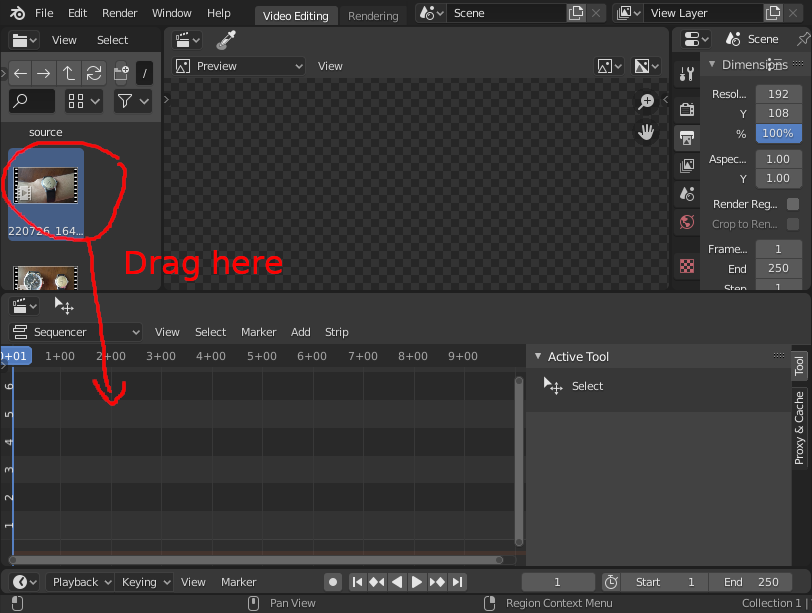
\includegraphics[scale=0.3]{image202209/blender_import.png}
\end{center}

デフォルトでは最終のフレームが 250 になっています。このままだと、動画が途中で終了したり、余分な黒画面が表示されてしまうので
適当な値を入力して変更してください。

\begin{center}
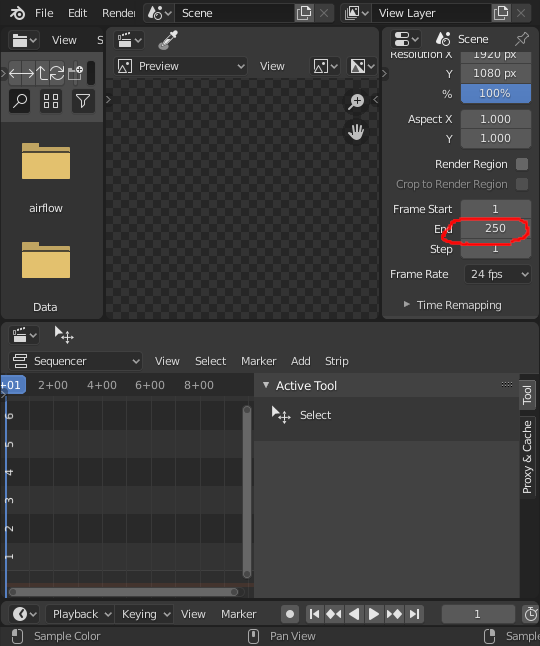
\includegraphics[scale=0.3]{image202209/blender_change_end.png}
\end{center}

\subsubsection{タイミングを合せる}

マウスでシーケンサのカラーバーをドラッグすると、対象が表示されるタイミングが調節できます。
カラーバーの端をクリックすると延長/短縮できるモードに切り替ります。

また、シーケンサー上で上下にドラッグする事で、チャンネルを変更する事ができます。
動画、画像、ナレーションやBGMなど、それぞれのチャンネルに分けておいた方が整理できます。

\begin{center}
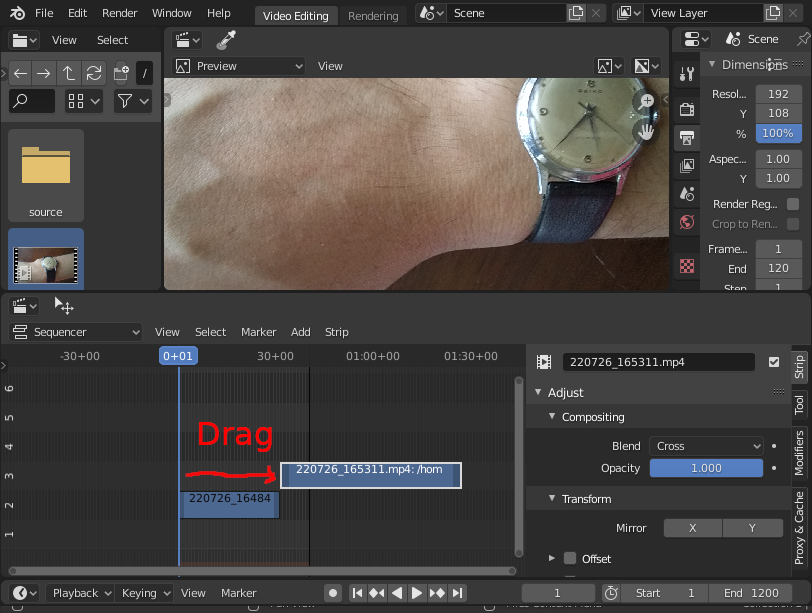
\includegraphics[scale=0.3]{image202209/blender_change_start_frame.png}
\end{center}

しかし、これよりも開始と終了のフレーム数を指定した方が良いと思います。
シーケンサで対象をクリックして選択すると、対象のパラメタが右下のメニューに表示されます。
ここで Start もしくは End に希望するフレーム数を入力してください。

\begin{center}
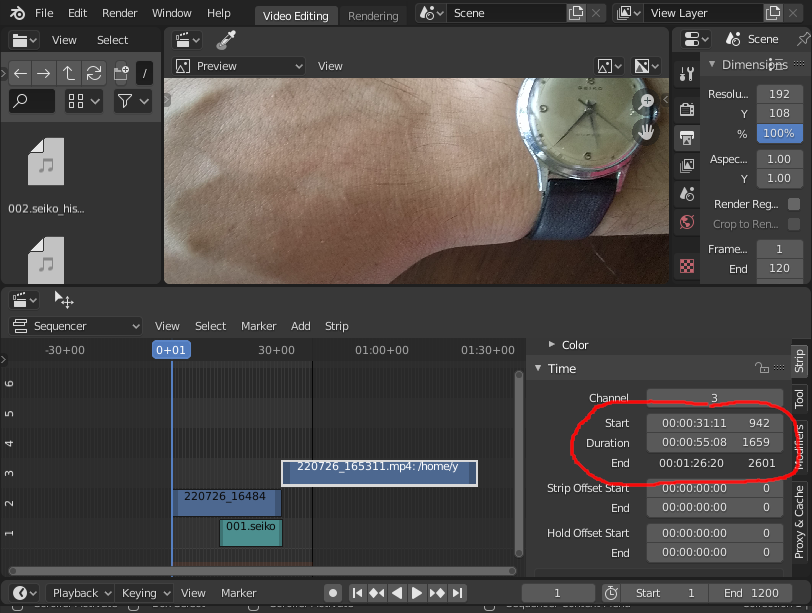
\includegraphics[scale=0.3]{image202209/blender_change_time_frame.png}
\end{center}

\subsubsection{動画に文字を入れる}

シーケンサの上、中段のメニューにある [add/text] を選択すると、
シーケンサに text オブジェクトが生成さます。

テキストの替りに、ロゴなどを入れたい場合は画像としてインポートできます。
gimp で画像を作成、または加工してください

\begin{center}
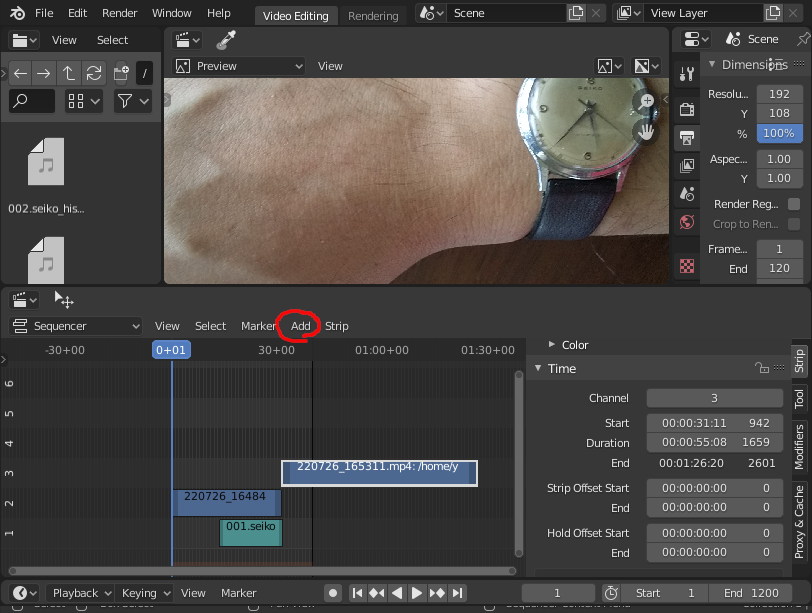
\includegraphics[scale=0.3]{image202209/blender_add_text.png }
\end{center}

text オブジェクトを選択して、パラメタを編集します。
Effect Strip (赤枠)に表示したい文字列を入力し、
Style (黄枠) で文字のサイズと色を調節します。
そして、Layout (青枠) で文字の位置を調節しましょう。

\begin{center}
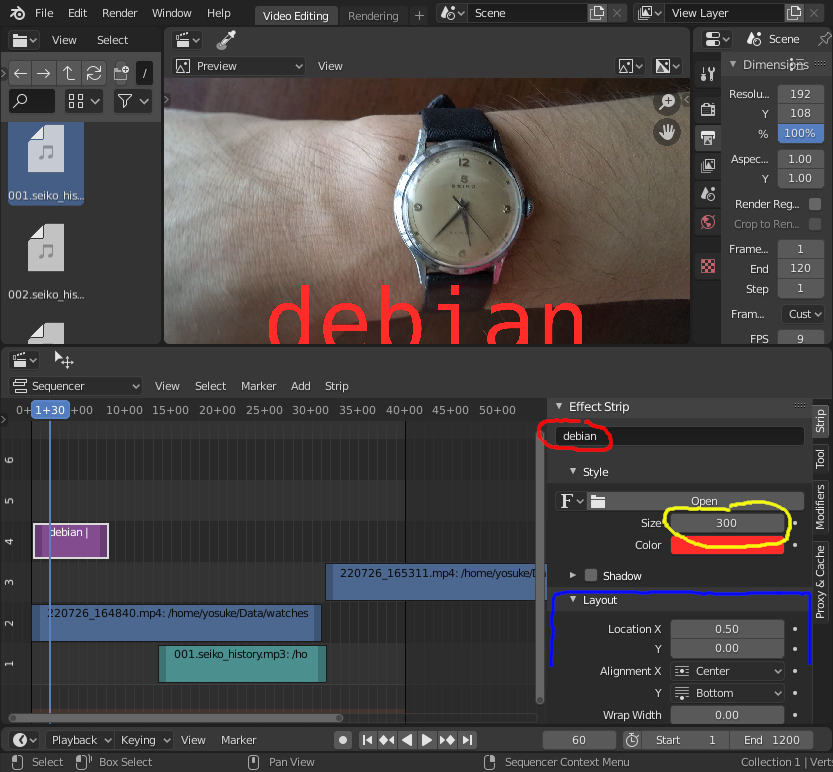
\includegraphics[scale=0.3]{image202209/blender_text_params.png }
\end{center}

\subsubsection{編集した動画を出力する}

debian 版の bledner は、動画と音声を合成して 1 つの動画ファイルとして出力することができません。\footnote{アップストリーム版は未確認}
そのため、動画ファイルの出力と音声ファイルの出力を別々に行い、
ffmpeg で合成します。

まずは出力する動画のフォーマットを決めます。
デフォルトで full HD の 24 fps になっているので YouTube などにアップロードする場合は変更する必要はないと思います。
変更する場合は、dimension の横のアイコンをクリックすると、任意のサイズを選択できます。

\begin{center}
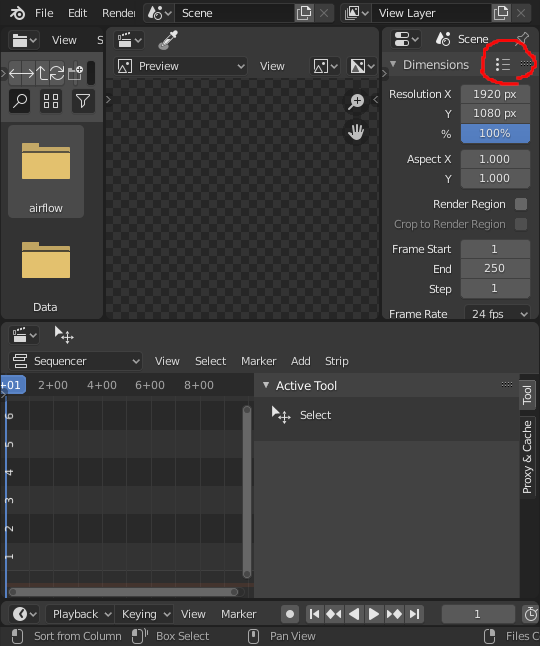
\includegraphics[scale=0.3]{image202209/blender_video_size.png}
\end{center}

また、少しスクロールしていくと [Frame Rate] という入力があります。
業界のデファクトスタンダードとして、YouTube が 24fps, 映画が 30fps, 特殊用途の動画が 60fps らしいです。 

次に、編集した動画をファイル出力します。
右上段のメニューに、[Output] というファイルパスがあります。
それが動画ファイルの出力先です。デフォルトでは /tmp になっています。

\begin{center}
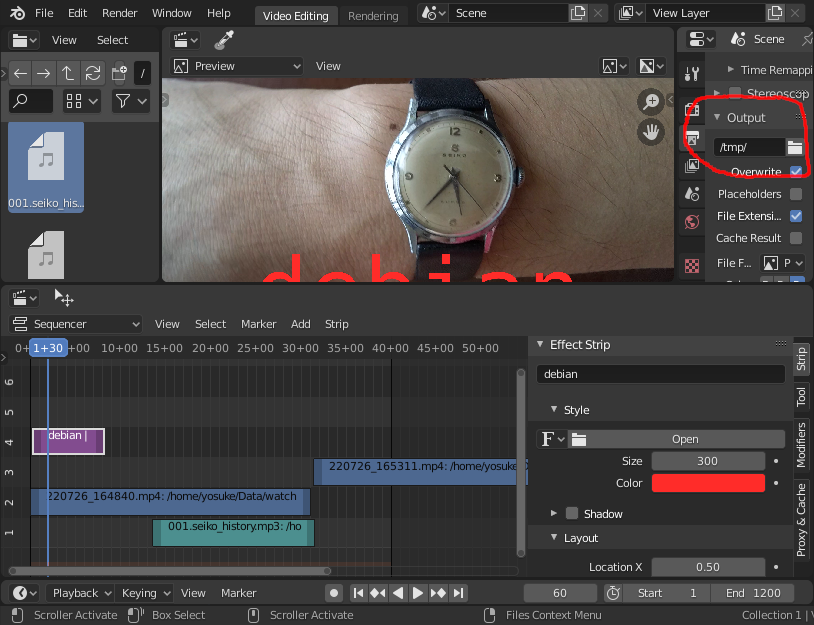
\includegraphics[scale=0.3]{image202209/blender_output.png}
\end{center}

また、File Format も PNG になっているので動画ファイル形式に変更しましょう。
ffmpeg video 形式で良いと思います。

\begin{center}
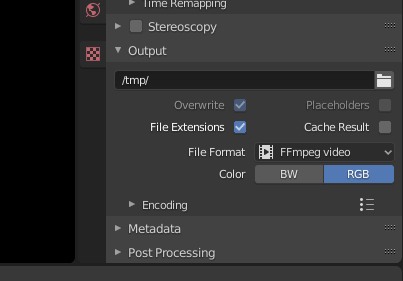
\includegraphics[scale=0.3]{image202209/blender_output_params.png}
\end{center}

動画の出力はトップのメニューバーから [Render/Render Animation] を押下してください。

\subsubsection{編集した音声を出力する}

今度は、音声ファイルを出力します。
[Render/Render Audio] を選択し、出力先をしていしたら、[Mix Down] ボタンを押下してください。 

\subsubsection{ffmpeg で出力した動画と音声を合成する}

blender から出力した動画と音声を ffmpeg で合成します

\begin{commandline}
ffmpeg -i ${movie_file} -i ${sound_file} -c:v copy -c:a aac ${output}
\end{commandline}

\subsection{番外編}
\subsubsection{その他のツール}
\begin{description}
\item{OBS:
たぶん知名度は No.1。ストリーミングから、動画の録画までできる。
しかし、動画の編集機能はない(はず)。
Podcast や雑談などを録画するには良い。debian 11 では パッケージ化済}
\vspace{1em}

\item{Natron:
動画編集用のソフトウェア、Blender の代りに使用できる。
Adobe の After Effect と同じような、node + edge で編集する仕様らしい。この仕様がハイエンドには多いとか...(未確認)
プロ用の動画編集ソフトウェアを使用した経験がなかったので、使用しなかった。
慣れている人には、学習コストが低いかもしれない。debian 11 ではパッケージ化はされていない。
アップストリームからバイナリをインストールするのが、エンコードがかなり遲かった。
ローカルでビルドしても良いかも}
\vspace{1em}

\item{Openshot:
こちらも動画編集用のソフトウェア Blender を代替できる。debian 11 では パッケージ化済
触った感じでは、blender よりも学習コストは低そう}
\vspace{1em}

\item{DaVinCi Resolve:
これだけ、OSS ではない。プロ用のハイエンドだが無料版がある。Win, Mac と Linux のバイナリが公式から入手可能。インストールしてみたが Nvidia の GPU が必須で起動ができなかった}
\vspace{1em}

\item{OpenjTalk:
OSS ゆっくり動画っぽいものを作成する場合は、OpenJTalk を使用する方法もあります}
\vspace{1em}

\end{description}
%\subsubsection{ナレーションを合成音声で生成する}
%OpenjTalk という音声合成ソフトウェアがあるので紹介します。

% 冊子にするために、4の倍数にする必要がある。
% そのための調整
%\dancersection{メモ}{}
%\mbox{}\newpage

\vspace*{15cm}
\hrule
\vspace{2mm}

\includegraphics[width=2cm]{image-assets/openlogo-nd.eps}
\noindent \Large \bf Debian 勉強会資料\\
\noindent \normalfont \debmtgyear{}年\debmtgmonth{}月\debmtgdate{}日 \hspace{5mm}  初版第1刷発行\\
\noindent \normalfont 東京エリア Debian 勉強会 (編集・印刷・発行)\\
\hrule
\end{document}
